\documentclass{beamer}
\usetheme{Frankfurt}
\usepackage[utf8]{inputenc}
\usepackage{charter}
\usepackage{tikz}
\usepackage{graphicx}
\usepackage{amsmath}
\usepackage{amssymb}
\usepackage{listings}
\usepackage{animate}
\usepackage{bm}
\usepackage{mathtools}
\usepackage{physics}
\mathtoolsset{showonlyrefs}
\beamertemplatenavigationsymbolsempty

\let\vec\bm

%% Title slide formatting %%

\pgfdeclareimage[width=\paperwidth]{titlebackground}{Images/title-slide-background.png}
\setbeamerfont{subtitle}{size=\tiny}
\setbeamertemplate{endpage}{
	\begin{picture}(0,0)
		\scalebox{1.01}{
		\put(-28.5,-163){%
			\pgfuseimage{titlebackground}
		}
		}
		\put(0,-115){%
			\begin{minipage}[b][4.5cm][t]{0.5\textwidth}
				\color{white}
				\usebeamerfont{title}
				{\textbf{Thank Your} \\ \textbf{For You Attention !}}
			\end{minipage}
		}
	\end{picture}
}
\setbeamertemplate{title page}{
	\begin{picture}(0,0)
		\scalebox{1.01}{
			\put(-28.5,-163){%
				\pgfuseimage{titlebackground}
			}
		}
		\put(0,-75){%
			\begin{minipage}[b][4.5cm][t]{0.7\textwidth}
				\color{white}
				\usebeamerfont{title}
				{\inserttitle\\[0.9cm]}
				\usebeamerfont{subtitle}
				{\insertauthor\par}
				{\insertinstitute\\[0.3cm]}
				{\insertdate}
			\end{minipage}
		}
	\end{picture}
}


%% General slide formatting %%

\definecolor{oxfordblue}{RGB}{4,30,66}

\pgfdeclareimage[width=0.9cm]{oxfordlogo}{Images/oxford-logo.png}
\pgfdeclareimage[width=1cm]{mathslogo}{Images/mathematics-logo.png}
\pgfdeclareimage[width=0.9cm]{pizzalogo}{Images/pizza-logo.png}

\setbeamertemplate{headline}
{%
	\begin{picture}(0,0)
		\put(314,-50){%
			\pgfuseimage{oxfordlogo}
		}
		\put(20,-55){%
			\rule{320pt}{0.4pt}
		}
	\end{picture}
}

\setbeamertemplate{frametitle}
{%
	\begin{picture}(0,0)
		\put(-8,-20){%
			\normalsize\textbf{\color{oxfordblue}\insertframetitle}
		}
		\put(-8,-32){%
			\normalsize\textbf{\color{oxfordblue}\insertframesubtitle}
		}
	\end{picture}
}

\setbeamertemplate{footline}
{%
	\begin{picture}(0,0)
		\put(20,30){%
			\rule{320pt}{0.4pt}
		}
		\put(20,14){%
			\pgfuseimage{mathslogo}
		}
		\put(100,14){%
			\color{oxfordblue}\insertshortdate
		}
		\put(160,14){%
			\color{oxfordblue}\insertshorttitle
		}
		\put(337,14){%
			\color{oxfordblue}\insertpagenumber
		}
	\end{picture}%
}
\setbeamercolor{block title}{bg=oxfordblue!30,fg=black}

\definecolor{codegreen}{rgb}{0,0.6,0}
\definecolor{codegray}{rgb}{0.5,0.5,0.5}
\definecolor{codepurple}{rgb}{0.58,0,0.82}
\definecolor{backcolour}{rgb}{0.95,0.95,0.92}

\lstdefinestyle{mystyle}{
	%backgroundcolor=\color{backcolour},   
	commentstyle=\color{codegray},
	keywordstyle=\color{oxfordblue},
	numberstyle=\tiny\color{codegray},
	stringstyle=\color{codegreen},
	basicstyle=\ttfamily\footnotesize,
	breakatwhitespace=false,         
	breaklines=true,                 
	captionpos=b,                    
	keepspaces=true,                 
	numbers=left,                    
	numbersep=5pt,                  
	showspaces=false,                
	showstringspaces=false,
	showtabs=false,                  
	tabsize=2
}

\lstset{style=mystyle}

%% Information (author, title, etc.) %%
\title[Acoustic Rarefied Nematic Liquid Crystals]{Anisotropic Acoustic Waves \vspace{0.2cm}\\ In Rarefied Nematic Liquid Crystals} % short title for footer
\author%
{%
	\sc{P. E. Farrell} *, \underline{\sc{U. Zerbinati}} *\\
}
\institute%
{%
	* \textit{Mathematical Institute}\\
	\;\textit{University of Oxford}\\
}

\date[Firedrake 2023]{22nd GAMM Seminar on Microstructures, 27th of January 2023, Vienna} % short date for footer



%% Content of slides %%

\begin{document}
	\begin{frame}[plain]
		\titlepage
	\end{frame}
	%
	\begin{frame}
		\frametitle{Why Rarefied Nematic Liquid Crystal ?}
		\begin{minipage}{0.49\textwidth}
			\vspace{0.8cm}
			\begin{figure}
				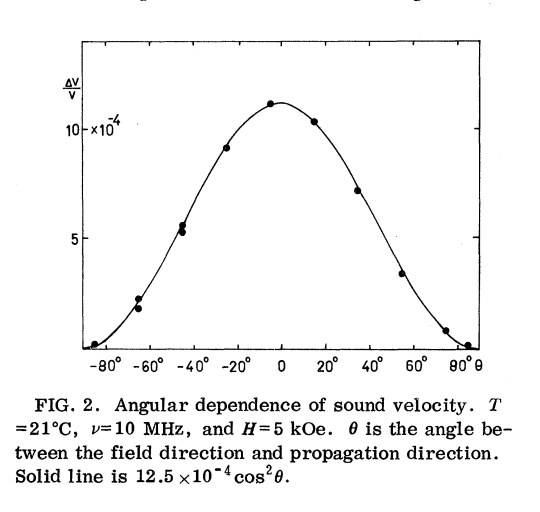
\includegraphics[scale=0.25]{Figures/MullenLuthiStephen}
				\vspace{-0.4cm}
				\caption{It was observed in \cite{MullenEtAll} that acoustic waves travel in NLC faster in the direction parallel to the nematic director.}
			\end{figure}
		\end{minipage}
		\begin{minipage}{0.49\textwidth}
			\vspace{1cm}
			\begin{figure}
				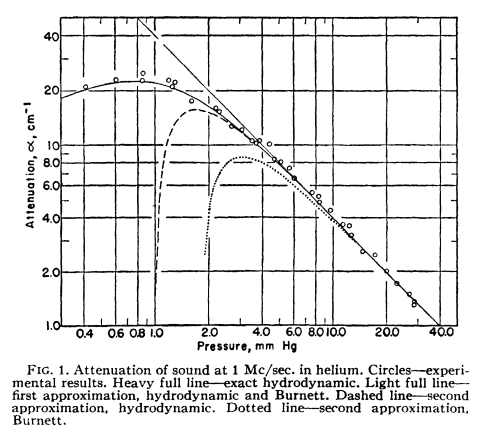
\includegraphics[scale=0.25]{Figures/Greenspan}
				\caption{It was observed in \cite{Greenspan} that first order theory better fit experimental data on acoustic attenuation at low pressure.}
			\end{figure}
		\end{minipage}
	\end{frame}
	\begin{frame}
		\frametitle{Curtiss Collision Operator}
		$\newline$
		Curtis in his seminal paper \cite{Curtiss} proposed a kinetic theory for spherocylindrical molecules as an idealisation of polyatomic gas.
		\\
		$\newline$
		\begin{minipage}{0.7\textwidth}
			\begin{itemize}
				\item[\color{oxfordblue}$\blacktriangleright$] His considered a larger configuration space made by \textbf{position}, \textbf{velocity}, \textbf{Euler's angles} for describing the orientation of each molecules and the \textbf{angular velocity} with respect to a fixed coordinate system.
				\item[\color{oxfordblue}$\blacktriangleright$] Molecules would interact by \textbf{excluded volume}, which give rise to \textbf{short range interactions} hence the \textbf{nematic ordering}.
			\end{itemize}
		\end{minipage}
		\qquad
		\begin{minipage}{0.2\textwidth}
			\begin{figure}
				\centering
				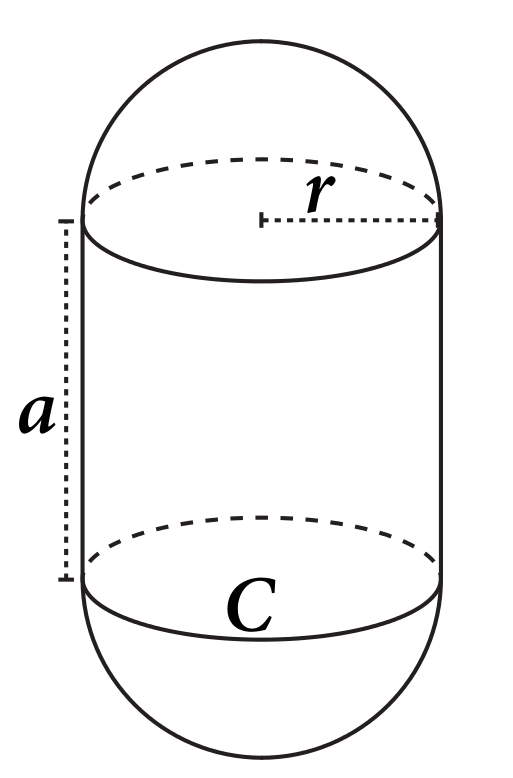
\includegraphics[scale=0.15]{Figures/spherocylinder}
			\end{figure}
		\end{minipage}
	\end{frame}
	\begin{frame}
		$\newline$
		$\newline$
		$\newline$
		This led Curtiss to formulate the following \textbf{Boltzmann} type equation,
		\begin{equation}
			\partial_t f + \nabla_{\vec{r}}\cdot(\vec{v}f)+\nabla_{\vec{\alpha}}\cdot(\dot{\vec{\alpha}}f) = C[f,f]\label{eq:Boltzman}
		\end{equation}
		where $f(\vec{r},\vec{v},\vec{\alpha},\vec{\omega})$ is the usual first reduced distribution function and $C[f,f]$ is the collision operator defined as
		\begin{equation}
			C[f,f] = - \int\int\int\int (f_1^{'}f^{'}-f_1f)(\vec{k}\cdot\vec{g})S(\vec{k})d\vec{k}d\vec{v}_1d\vec{\alpha}_1d\vec{\omega}_1
		\end{equation}
		with $\S(\vec{k})d\vec{k}$ being the surface element of the excluded volume and $\vec{g}=\vec{v}-\vec{v}_1$.
		Here with out loss of generality the equation is stated in \textbf{absence of external force} and \textbf{torque}.
	\end{frame}
	\begin{frame}
		\frametitle{Collision Invariants}
		$\newline$
		$\newline$
		$\newline$
		It is possible to prove that the following quantities are \textbf{collision invariants} for $C[f,f]$, i.e.
		\begin{equation}
			\int\int\int \psi^{(i)}d\vec{v}_1d\vec{\omega}_1d\vec{\alpha}_1 = 0.
		\end{equation}
		\begin{itemize}
			\item[\color{oxfordblue}$\blacktriangleright$] $\psi^{(1)}=1$, the \textbf{number of particle} in the system;
			\item[\color{oxfordblue}$\blacktriangleright$] $\psi^{(2)}=m\vec{v}$, the \textbf{linear momentum};
			\item[\color{oxfordblue}$\blacktriangleright$] $\psi^{(3)}=\mathbb{I}\footnote{\vspace{1cm}The inertia tensor for the spherocylinder we are considering.}\cdot\omega+\vec{r}\times m\vec{v}$, the \textbf{angular momentum};
			\item[\color{oxfordblue}$\blacktriangleright$] $\psi^{(4)}=\frac{1}{2}m\vec{v}\cdot \vec{v} + \frac{1}{2}\vec{\omega}\cdot\mathbb{I}\cdot\vec{\omega}$, the \textbf{kinetic energy of the system}.
		\end{itemize}
	\end{frame}
	\begin{frame}
		$\newline$
		$\newline$
		\frametitle{The Hydrodynamic Equations -- Notation}
		We first introduce the \textbf{number density}, i.e.
		\begin{equation}
			n(\vec{r})= \int\int\int f(\vec{r},\vec{v},\vec{\alpha},\vec{\omega}) d\vec{v}d\vec{\alpha}d\vec{\omega}.
		\end{equation}
		Then we can give a meaning to the following \textit{chevrons}, i.e.
		\begin{equation}
			\langle\langle\cdot \rangle\rangle(\vec{r}) = \frac{1}{n(\vec{r})}\int\int\int \cdot\; f(\vec{r},\vec{v},\vec{\alpha},\vec{\omega}) d\vec{v}d\vec{\alpha}d\vec{\omega}.
		\end{equation}
		Using this notation we can define \textbf{macroscopic stream velocity} and \textbf{macroscopic stream angular velocity} respectively as:
		\begin{equation}
			\vec{v}_0 := \langle\langle \vec{v} \rangle\rangle, \qquad \vec{\omega}_0 := \langle\langle \vec{\omega} \rangle\rangle.
		\end{equation}
	\end{frame}
	\begin{frame}
		$\newline$
		$\newline$
		\frametitle{The Hydrodynamic Equations -- Curtis Balance Laws}
		Testing \eqref{eq:Boltzman} against the first two \textbf{collision invariants} and integrating  Curtis obtained the following \textbf{balance laws}:
		\begin{equation}
			\partial_t\rho + \nabla_{\vec{r}}\cdot(\rho\vec{v}_0)\label{eq:KT1}=0,
		\end{equation}
		\begin{equation}
			\rho \Big[\partial_t \vec{v}_0 + (\nabla_{\vec{r}}\vec{v}_0)\vec{v}_0\Big]+\nabla_{\vec{r}}\cdot(\rho \mathbb{P})=0,\label{eq:KT2}
		\end{equation}
		where $\rho$ is the \textbf{density} defined as $\rho(\vec{r})=mn(\vec{r})$ and $\mathbb{P}$ is the \textbf{pressure tensor} defined as $\mathbb{P}=\langle\langle\vec{V}\otimes \vec{V}\rangle\rangle$, with $V$ being the \textbf{peculiar velocity} $\vec{V}:=\vec{v}-\vec{v}_0$.
	\end{frame}
	\begin{frame}
		$\newline$
		$\newline$
		\frametitle{The Hydrodynamic Equations -- Surprise Balance Laws}
		For the third collision invariant we took a different rout then Curtis, which led to the following balance law
		\begin{equation}
			\rho \Big[\partial_t \vec{\eta} + (\nabla_{\vec{r}}\vec{\eta})\vec{v}_0\Big]+\nabla_{\vec{r}}\cdot(\rho \mathbb{N})=\vec{\xi},\label{eq:KT3}
		\end{equation}
		where $\vec{\eta}$ is the \textbf{macroscopic intrinsic angular momentum} defined as $\vec{\eta}(\vec{r})=\langle\langle \mathbb{I} \cdot \omega \rangle\rangle$ and $\mathbb{P}$ is the \textbf{couple tensor} defined as $\mathbb{N}=\langle\langle\vec{V}\otimes(\mathbb{I}\vec{\omega}\rangle\rangle$. Here $\vec{\xi}$ is defined in tensor notation as $\langle\langle mn(\varepsilon_{lki} v_iv_k)\vec{e}_l\rangle\rangle$ and we proved that $\vec{\xi}$ vanish (as stated by Curtis in \cite{Curtiss}) in this particular setting.
	\end{frame}
	\begin{frame}
		\frametitle{Maxwell-Boltzmann Distribution}
		$\newline$
		In \cite{Curtiss} Curtis gives an expression for the Maxwell-Boltzmann distribution, i.e. such distribution $f^{(0)}$ such that $C[f^{(0)},f^{(0)}]$ vanish.
		\begin{equation}
			f^{(0)} (\vec{v},\vec{\omega}) = n \frac{\sin(\alpha_2)Q}{\int Q \sin(\alpha_2)d\vec{\alpha}}\frac{m^{\frac{3}{2}}}{2\pi \theta}^3(\Gamma_1\Gamma_2\Gamma_3)^{\frac{1}{2}}\exp\Big[-m\frac{\abs{\vec{V}}}{2\theta}-\frac{\vec{\Omega}\cdot\mathbb{I}\cdot\vec{\Omega}}{2\theta}\Big]
		\end{equation}
		where the \textbf{peculiar angular velocity} defined as $\vec{\Omega}=\vec{\omega}-\vec{\omega}_0$, $\Gamma_i$ are the moments of inertia of the spherocylinder we are considering and $Q$ is defined as $Q = \exp\Big[\frac{\vec{\omega}_0\cdot\mathbb{I}\cdot\vec{\omega}_0}{2\theta}\Big]$.\\
		\vspace{0.2cm}
		Notice in particular that we assumed $\vec{\omega}_0$ and the \textbf{kinetic temperature} $\theta = \langle\langle \frac{m}{2}\vec{V}\cdot \vec{V}+\frac{1}{2}\vec{\Omega}\cdot \mathbb{I}\cdot \vec{\Omega}\rangle\rangle$ are fixed.
	\end{frame}
	\begin{frame}
		\frametitle{Momentum Closure Around The Equilibrium}
		$\newline$
		$\newline$
		Now we can use the previous distribution to compute an approximation of the \textbf{pressure tensor} near the equilibrium, i.e.
		\begin{equation}
			\mathbb{P}^{(0)} = \theta \vec{Id}
		\end{equation}
		We can define the \textbf{pressure} as $p=\rho\theta\footnote{\vspace{0.8cm}This shows that the pressure is a monotonically increasing function of the density which is needed in order to have a positive speed of sound.}$ and rewrite,
		\begin{equation}
			\Big[\partial_t \vec{v}_0 + (\nabla_{\vec{r}}\vec{v}_0)\vec{v}_0\Big]=-\frac{1}{\rho}\nabla p,\label{eq:KTEuler}
		\end{equation}
		which is the well known \textbf{Euler equation} that if linearised yield the \textbf{wave equation}.\\{\color{red}\textbf{Unfortunately}} same procedure result in a {\color{red}\textbf{vanishing}} $\mathbb{N}^{(0)}$.
	\end{frame}
	\begin{frame}
		\frametitle{Balance Laws For Kinetic Temperature}
		$\newline$
		We need an other way to formulate \textbf{constitutive relation} for the \textbf{couple tensor}, we begin observing that testing $\psi^{(4)}$ we get the following balance law:
		\begin{equation}
			\dot{\psi} + \nabla_{\vec{r}}\vec{v}_0:\mathbb{P}+\nabla_{\vec{r}}\vec{\omega}_0:\mathbb{N} - \nabla\cdot\Big[\mathbb{P}^T\vec{v}_0+\mathbb{N}^T\vec{\omega}_0\Big]\geq 0
		\end{equation}
		where $\psi = \langle\langle \theta \rangle\rangle$.
		We add $\vec{\xi}$ and observe that if we integrate with appropriate boundary condition the expression is the \textbf{rate of work} theorem that was the starting point of Leslie-Ericksen theory
		\begin{equation}
			\dot{\psi} + \nabla_{\vec{r}}\vec{v}_0:\mathbb{P}+\nabla_{\vec{r}}\vec{\omega}_0:\mathbb{N} - \nabla\cdot\Big[\mathbb{P}^T\vec{v}_0+\mathbb{N}^T\vec{\omega}_0\Big]+{\color{red}\vec{\xi}}\geq 0\label{eq:PowerExpanded}
		\end{equation}
	\end{frame}
	\begin{frame}
		\frametitle{Noll--Coleman Procedure}
		$\newline$
		Since we are happy with our \textbf{pressure tensor} so far we make the following \textbf{ansatz}
		\begin{equation}
			\psi = \psi(\nu,\nabla\nu)
		\end{equation}
		where $\nu$ is the \textbf{nematic director}. Expanding the total derivative and using Ericksen identity we get the following expression in tensor notation
		\begin{align}
			\dot{\psi} = \varepsilon_{iqp}\Big[(\nu_q \frac{\partial\psi}{\partial(\nu_p)}+\partial_k(\nu_q)\frac{\partial\psi}{\partial(\partial_k\nu_p)})\omega^0_i&+\nu_q\frac{\partial\psi}{\partial(\partial_k\nu_p)}\partial_k\omega^0_i\Big]\\&-\frac{\partial\psi}{\partial(\partial_k\nu_p)}\partial_q(\nu_p)\partial(v^0_q)
		\end{align}
	\end{frame}
	\begin{frame}
		\frametitle{Noll--Coleman Procedure}
		$\newline$
		$\newline$
		Substituting this expression inside of \eqref{eq:PowerExpanded} and considering thermodynamic process for which the exact divergences disappear we get:
		\vspace{-0.3cm}
		\begin{align}
			\Big[\mathbb{P}_{ij}+\frac{\partial\psi}{\partial(\partial_j\nu_p)}\partial_i(\nu_p)\Big]\partial_j(\nu_i)&+\Big[N_{ij}-\varepsilon_{iqp}\nu_q\frac{\partial \psi}{\partial(\partial_j \nu_p)}\Big]\partial_j(\omega^0_i)\\
			&\Big[P_{pq}-\frac{\partial\psi}{\partial(\partial_p\nu_k)\partial_q(\nu_k)}\Big]\varepsilon_{iqp}\omega^0_i\geq0\label{eq:NollColeman}
		\end{align}
		Once again since the above expression must hold for all thermodynamic process for which the exact divergences disappear we get the following \textbf{constitutive relations}:
		\vspace{-0.3cm}
		\begin{equation}
			\mathbb{P} = \nabla\vec{\nu}^T \frac{\partial\psi}{\partial(\nabla\vec{\nu})}+\mathbb{P}^{(0)}, \qquad N_{ij} = \varepsilon_{iqp} \nu_q \frac{\partial\psi}{\partial(\partial_j\nu_p)}={\color{red}\vec{\nu} \times\frac{\partial\psi}{\partial(\nabla\vec{\nu})}}
		\end{equation}
	\end{frame}
	\begin{frame}
		\frametitle{Anisotropic Waves}
		$\newline$
		It can be showed that steady spherical solution of \eqref{eq:KT3} are of the form $\vec{\nu} = \frac{\vec{r}}{\abs{\vec{r}}}$ and that $\nabla\vec{\nu}^T\nabla\vec{\nu} = \vec{Id}-\vec{\nu}\otimes\vec{\nu}$. Therefore for this particular case we have the following choice of \textbf{pressure tensor}:
		\begin{equation}
			\mathbb{P} = \mathbb{P}^{(0)}+\vec{Id}+\vec{\nu}\otimes\vec{\nu}.
		\end{equation}
		If we linearise the \textbf{Euler equation} with this choice of \textbf{pressure tensor} we get the eave equation:
		\begin{equation}
			\partial_t^2p - \nabla\cdot \Big[(\vec{Id}+\vec{\nu}\otimes\vec{\nu})\nabla p\Big]=0.
		\end{equation}
	\end{frame}
	\begin{frame}
		\frametitle{Anisotropic Waves}
		And it is well known that when we have a planer wave 
		\begin{equation}
			p(\vec{r},t) = A\cos(\vec{k}\cdot\vec{r}-\omega t)
		\end{equation}
		travelling in a transversely isotropic medium has speed of sound
		\begin{equation}
			\boxed{c_s =  (1+cos(\theta))^2}
		\end{equation}
		where $\theta$ is the angle between $\vec{k}$ and $\vec{\nu}$.
	\end{frame}
	\begin{frame}[t, allowframebreaks]
		\frametitle{References}
		$\newline$
		$\newline$
		\bibliographystyle{amsalpha}
		\bibliography{metrix}
	\end{frame}
\end{document}
